\documentclass[12pt]{article}

\usepackage[T1]{fontenc}
\usepackage[utf8]{inputenc}
\usepackage{polski}
\usepackage{amssymb, amsfonts, amsmath}
\usepackage{graphicx}
\usepackage{verbatim}
\usepackage{hyperref}
\usepackage{enumerate}
\usepackage{blindtext}
\usepackage{float}
\begin{document}
\title{Projekt aplikacji do analizy i wizualizacji danych dotyczących wrażeń synestetycznych}
\author{Łukasz Brzozowski}
\maketitle
\begin{figure}[ht!]
	\centering
	
\includegraphics[width=\textwidth]{MiNI.png}
\end{figure}
\begin{figure}[ht!]
	\centering
	
\includegraphics[width=8cm]{Pw.png}
\end{figure}
\pagebreak
\section{Opis problemu}
	Celem projektu jest stworzenie aplikacji, która na podstawie danej próbki tekstu będzie dynamicznie tworzyć animacje mające odwzorować wrażenia osób z przypadłością synestezji wzrokowo-leksykalnej. Dzięki takiej aplikacji nastąpi zwiększenie się świadomości społecznej dotyczącej synestezji oraz będzie możliwe przedstawienie codzienności osób z ową cechą. Ponadto, na podstawie danych zebranych od synestetyków zostanie przeprowadzona analiza połączeń kolorystyczno-literowych umożliwiająca odnalezienie najczęstszych wzorców oraz schematów przyporządkowania kolorów.
\begin{figure}[ht!]
	\centering
	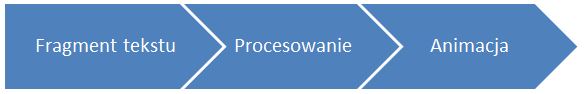
\includegraphics[width=10cm]{Capture.PNG}
	\caption{Działanie aplikacji}
\end{figure} 
\begin{figure}[ht!]
	\centering
	\fbox{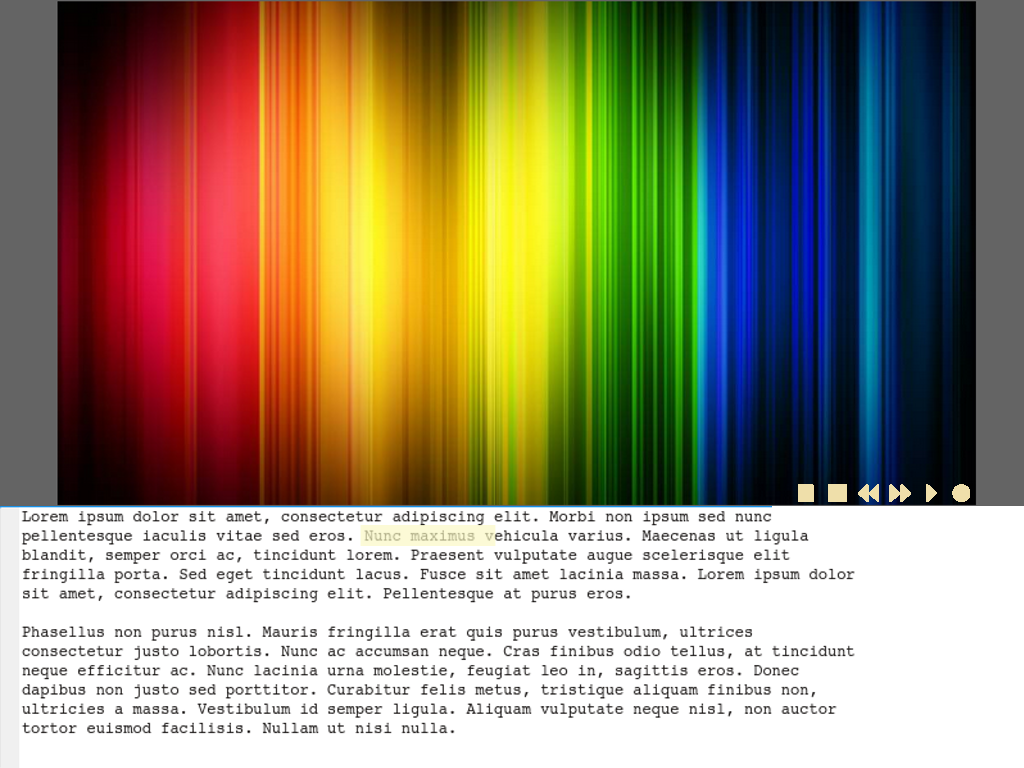
\includegraphics[width=11cm]{Prototyp_programu.png}}
	\caption{Przykładowy interfejs aplikacji dynamicznie tworzącej animacje}
\end{figure}
\pagebreak
\section{Analiza istniejących rozwiązań}
Na tę chwilę nie są dostępne żadne narzędzia służące do wizualizacji wrażeń synestetycznych wynikających z powiązań wzrokowo-leksykalnych. Można jednak znaleźć aplikacje animujące wrażenia wzrokowo-słuchowe. Bazują one na indywidualnych skojarzeniach tonacji muzycznych i barw instrumentów z kolorami. 
\begin{figure}[H]
	\centering
	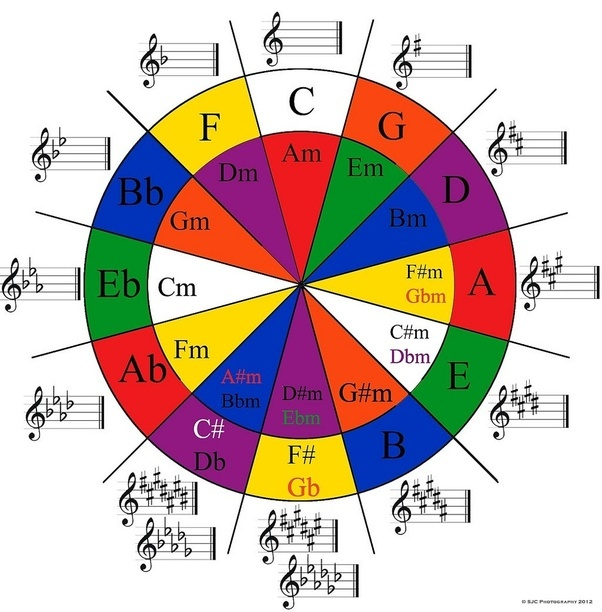
\includegraphics[width=11cm]{Bach.jpeg}
	\caption{Skojarzenia kolorów z tonacjami Jana Sebastiana Bacha}
\end{figure}
\pagebreak
Jedną z możliwych form wizualizacji jest przyporządkowanie kolorów klawiszom klawiatury fortepianu. Użytkownik serwisu YouTube o nicku aniMIDIfy napisał program w języu Python, korzystając również z oprogramowania FFMPEG, SoX, TiMidity, FluidSynth, Python Image Library oraz midicsv.
\begin{figure}[H]
	\centering
	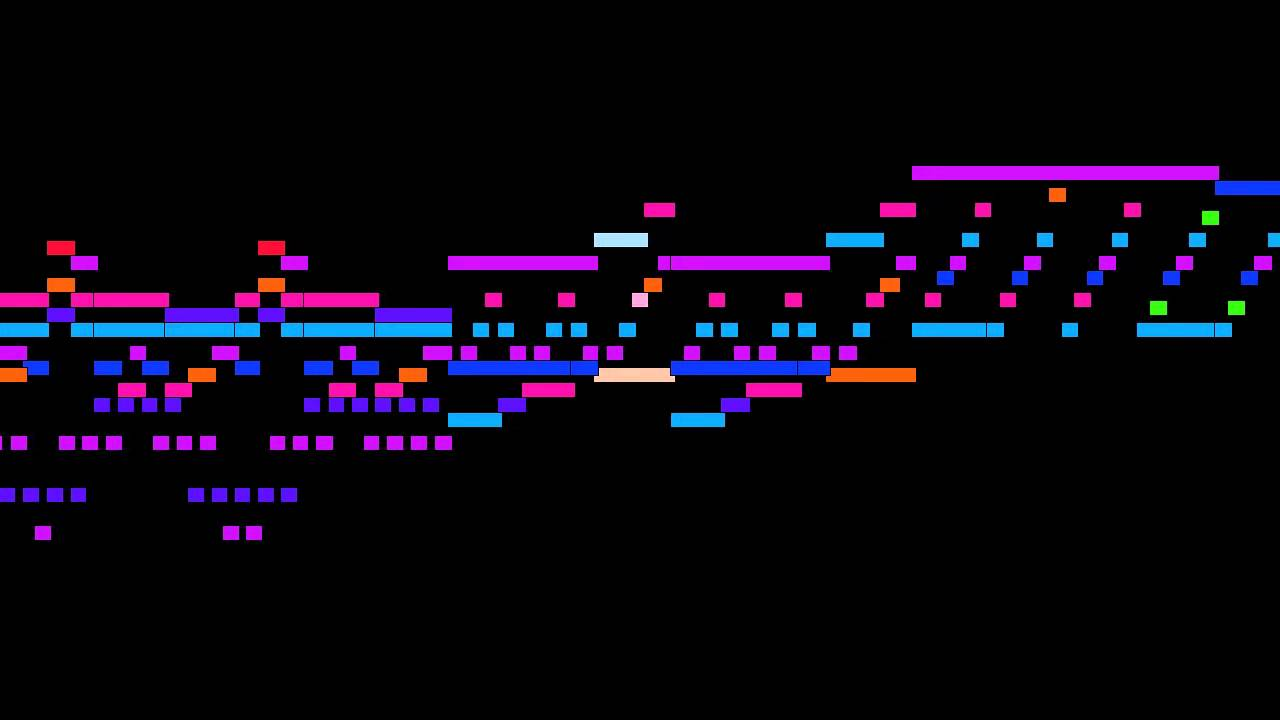
\includegraphics[width=\textwidth]{animidify.jpg}
	\caption{Klatka animacji z jednego z filmów użytkownia aniMIDIfy}
\end{figure}
\end{document}
